%%%%%%%%%%%%%%%%%%%%%%%%%%%%%%%%%%%%%%%%%%%%%%%%%%%%%%%%%%%%
%%  This Beamer template was created by Cameron Bracken.
%%  Anyone can freely use or modify it for any purpose
%%  without attribution.
%%
%%  Last Modified: January 9, 2009
%%

\documentclass[xcolor=x11names,compress]{beamer}

%% General document %%%%%%%%%%%%%%%%%%%%%%%%%%%%%%%%%%
\usepackage{graphicx}

\usepackage{xcolor}

\usepackage{pgffor} 

\usepackage{tikz}
\usetikzlibrary{shapes.callouts}

\usepackage{pgfplots}

%%%%%%%%%%%%%%%%%%%%%%%%%%%%%%%%%%%%%%%%%%%%%%%%%%%%%%

\usepackage[frenchb]{babel}

\usepackage[utf8]{inputenc}

\usepackage{lastpage}

\usepackage[natbib=true, bibstyle=authoryear,
citestyle=authoryear]{biblatex}

\usepackage{caption}
\captionsetup{figurename=}

\usepackage{appendixnumberbeamer}

\resetcounteronoverlays{lstnumber}

%% Beamer Layout %%%%%%%%%%%%%%%%%%%%%%%%%%%%%%%%%%
\useoutertheme[subsection=false,shadow]{miniframes}
\useinnertheme{default} \usefonttheme{serif} \usepackage{palatino}

\setbeamerfont{title like}{shape=\scshape}
\setbeamerfont{title}{shape=\scshape}
\setbeamerfont{frametitle}{shape=\scshape}
\setbeamerfont{footline}{shape=\scshape}

\definecolor{MRed}{HTML}{8B0000} \definecolor{MGreen}{HTML}{008B00}
\definecolor{MBlue}{HTML}{00688B}

\setbeamercolor*{lower separation line head}{bg=MBlue}
\setbeamercolor*{normal text}{fg=black,bg=white}
\setbeamercolor*{alerted text}{fg=red} \setbeamercolor*{example
  text}{fg=black} \setbeamercolor*{structure}{fg=black}

\setbeamercolor*{palette tertiary}{fg=black,bg=black!10}
\setbeamercolor*{palette quaternary}{fg=black,bg=black!10}

\setbeamercolor{footlinerule}{bg=MBlue}
\setbeamercolor*{footlinecolor}{bg=black!10}

\setbeamercolor{block title}{use=structure,fg=white,bg=MBlue!75!black}
\setbeamercolor{block body}{use=structure,fg=black,bg=MBlue!20!white}

\setbeamercolor{block title
  example}{use=structure,fg=white,bg=MGreen!75!black}
\setbeamercolor{block body
  example}{use=structure,fg=black,bg=MGreen!20!white}

\setbeamercolor{block title
  alerted}{use=structure,fg=white,bg=MRed!75!black}
\setbeamercolor{block body
  alerted}{use=structure,fg=black,bg=MRed!20!white}

\renewcommand{\(}{\begin{columns}} \renewcommand{\)}{\end{columns}}
\newcommand{\<}[1]{\begin{column}{#1}} \renewcommand{\>}{\end{column}}
%%%%%%%%%%%%%%%%%%%%%%%%%%%%%%%%%%%%%%%%%%%%%%%%%%


\author{Arnaud Bletterer} \title{Outils multidimensionnels de
  déformation}

\newcommand{\mytext}{Outils multidimensionnels de déformation}

\graphicspath{{PresentationFigs/}}

%%%%%%%%%%%%%%%%%%%%%%%%%%%%%%%%%%%%%%%%%%%%%%%%%%%%%%
%%%%%%%%%%%%%%%%%%%%%%%%%%%%%%%%%%%%%%%%%%%%%%%%%%%%%%

\makeatother \setbeamertemplate{footline} {%
  \leavevmode
  \begin{beamercolorbox}[wd=\paperwidth,ht=1ex,dp=0ex,center]{footlinerule}
  \end{beamercolorbox}%



  \hbox{\begin{beamercolorbox}[wd=1\paperwidth,ht=2.5ex,dp=1.125ex,leftskip=.3cm,rightskip=.3cm]{footlinecolor}%
      \count1 = \linewidth \divide\count1 by \inserttotalframenumber

      \foreach \n in {1,...,\insertframenumber}{\hskip1.\count1}
      
\includegraphics[scale=0.06, viewport= 400 200 0 0]{cgogn}
   
  \end{beamercolorbox}
}

\hbox{\begin{beamercolorbox}[wd=.5\paperwidth,ht=2.5ex,dp=1.125ex,leftskip=.3cm,rightskip=.3cm]{footlinecolor}%
    \inserttitle
  \end{beamercolorbox}%

    \begin{beamercolorbox}[wd=.5\paperwidth,ht=2.5ex,dp=1.125ex,leftskip=.3cm,rightskip=.3cm]{footlinecolor}%
      \usebeamerfont{author in head/foot}\insertauthor\hfill
      \insertframenumber /\inserttotalframenumber
    \end{beamercolorbox}}%
  \vskip0pt%
} \makeatletter

%%%%%%%%%%%%%%%%%%%%%%%%%%%%%%%%%%%%%%%%%%%%%%%%%%%%%%
%%%%%%%%%%%%%%%%%%%%%%%%%%%%%%%%%%%%%%%%%%%%%%%%%%%%%%

\newcommand{\highlightR}[1]{%
  \colorbox{MRed!50}{$\displaystyle#1$}} \newcommand{\highlightB}[1]{%
  \colorbox{MBlue!50}{$\displaystyle#1$}}
\newcommand{\highlightG}[1]{%
  \colorbox{MGreen!50}{$\displaystyle#1$}}
\newcommand{\highlightO}[1]{%
  \colorbox{orange!50}{$\displaystyle#1$}}
\newcommand{\highlightV}[1]{%
  \colorbox{violet!50}{$\displaystyle#1$}}
\newcommand{\highlightGR}[1]{%
  \colorbox{gray!50}{$\displaystyle#1$}}


%%%%%%%%%%%%%%%%%%%%%%%%%%%%%%%%%%%%%%%%%%%%%%%%%%%%%%
%%%%%%%%%%%%%%%%%%%%%%%%%%%%%%%%%%%%%%%%%%%%%%%%%%%%%%

\bibliography{../Rapport/References/references.bib}
\begin{document}

%%%%%%%%%%%%%%%%%%%%%%%%%%%%%%%%%%%%%%%%%%%%%%%%%%%%%%
%%%%%%%%%%%%%%%%%%%%%%%%%%%%%%%%%%%%%%%%%%%%%%%%%%%%%%
\begin{frame}
  \title{Outils multidimensionnels de déformation\\~\\

    \begin{figure}
      \begin{center}
        
\includegraphics[scale=0.3]{uds-logo}~~~~~~~~~
        
\includegraphics[scale=0.15]{icube-logo}
      \end{center}
    \end{figure}
  } \author{Arnaud Bletterer \\ \textit{Université de Strasbourg}
    \vspace{-0.5cm} \date{\today} } \titlepage
\end{frame}


%%%%%%%%%%%%%%%%%%%%%%%%%%%%%%%%%%%%%%%%%%%%%%%%%%%%%%
%%%%%%%%%%%%%%%%%%%%%%%%%%%%%%%%%%%%%%%%%%%%%%%%%%%%%%
\section{\scshape Introduction}

\begin{frame}{Contexte}
  \begin{itemize}
  \item Objet
    \begin{itemize}
    \item Discrétisé en cellules (sommet, arête, face, volume)
    \end{itemize}
  \item Déformation spatiale
    \begin{itemize}
    \item Déformation de l'espace ambiant
    \item Manipulation à l'aide d'un outil
      \begin{itemize}
      \item Un outil est un objet
      \item Manipulation directe des points de contrôle
      \item Différentes caractéristiques (dimension, résolution, zone
        d'influence)
      \end{itemize}
    \item Indépendante de la représentation interne
    \end{itemize}
  \end{itemize}
\end{frame}

\begin{frame}{Création d'un outil multidimensionnel}
  \begin{alertblock}{Problèmes}
    \setbeamercolor{itemize item}{fg=MRed}
    \begin{itemize}
    \item Finesse d'une déformation liée au nombre de DDL
    \item Complexité en temps de calcul liée au nombre de DDL
    \item Déformation difficile avec certains outils
    \end{itemize}
  \end{alertblock}
  \begin{figure}[h]
    \begin{center}
      
\includegraphics[scale=0.15]{alligator-ferme}
      
\includegraphics[scale=0.15]{alligator-ouvert}
    \end{center}
    \caption{\citep{JBPS11}}
  \end{figure}
\end{frame}

\begin{frame}{Création d'un outil multidimensionnel}
  \begin{block}{Mélanger plusieurs outils}
    \begin{itemize}
    \item Différentes dimensions/résolutions
    \item Déformation lisse (au moins $C^1$)
    \item Choisir l'outil le plus adapté aux déformations à appliquer
    \end{itemize}
  \end{block}
  \begin{figure}[h]
    \begin{center}
      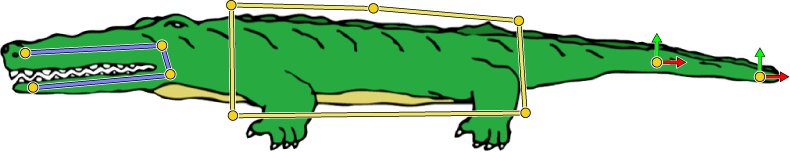
\includegraphics[scale=0.15]{alligator-avant}
      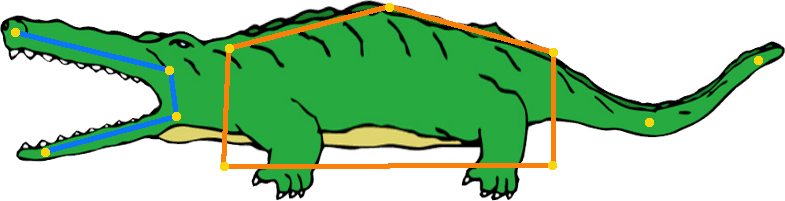
\includegraphics[scale=0.15]{alligator-apres}
    \end{center}
    \caption{\citep{JBPS11}}
  \end{figure}
\end{frame}


%%%%%%%%%%%%%%%%%%%%%%%%%%%%%%%%%%%%%%%%%%%%%%%%%%%%%%
%%%%%%%%%%%%%%%%%%%%%%%%%%%%%%%%%%%%%%%%%%%%%%%%%%%%%%
\section{\scshape Etat de l'art}

\begin{frame}{Outils existants}
  \begin{figure}[h]
    \begin{center}
      \begin{tabular}{|l|c|c|c|}
        \hline
        \textbf{Outil} & \textbf{Dim.} & \textbf{Type Def.} & \textbf{Forme du bord} \\
        \hline
        \hline
        Bézier & V & Globale & Cubique\\
        \hline
        Contrôle local & V & Locale & Cubique\\
        \hline
        Non-parallélépipédique & V & Locale & Libre\\
        \hline
        \hline
        Carreau paramétrique & S & Globale & Rectangulaire\\
        \hline
        Surface étoilée & S & Globale & /\\
        \hline
        Maillage triangulaire & S & Locale & Union de sphères\\
        \hline
        Cage & S & Globale & Libre\\
        \hline
        \hline
        Radiale simple & P & Locale & Union de sphères\\
        \hline
        DOGME & P & Locale & Cubique\\
        \hline
      \end{tabular}
      \caption{\citep{GB08}}
    \end{center}
  \end{figure}
\end{frame}

\begin{frame}{Etat de l'art}
  \begin{itemize}
  \item Bounded Biharmonic Weights for Real-Time Deformation
    $_{\text{\citep{JBPS11}}}$
  \item *Cages: A Multilevel, Multi-cage-based System for Mesh
    Deformation $_{\text{\citep{GPCP13}}}$
  \end{itemize}
\end{frame}

\begin{frame}{Bounded Biharmonic Weights $_{\text{\citep{JBPS11}}}$}
  \begin{itemize}
  \item Mélange d'outils de différentes dimensions
  \item Associer manuellement plusieurs outils sur différentes zones
    d'un même objet
  \item Méthode d'optimisation globale
    \begin{alertblock}{Points négatifs : }
      \setbeamercolor{itemize subitem}{fg=MRed}
      \begin{itemize}
      \item Déformation à base de points
      \item Contraintes sur le calcul des coordonnées
      \item Calcul des coordonnées par diffusion
      \end{itemize}
    \end{alertblock}
  \end{itemize}
\end{frame}

\begin{frame}{Déformation à base de cages}
  \begin{itemize}
\item $_{\text{\citep{JSW05}}}$ $_{\text{\citep{HF06}}}$
  \item Déformation globale
  \item Forme épousant celle de l'objet à déformer
  \end{itemize}
  \begin{equation}
    T(p) = \sum^n_{i=1} \lambda(c_i,p) \cdot c_i
  \end{equation}
  Où : \\
  $\lambda(c_i,p)$ est la coordonnée du point $p$ par rapport au
  sommet $c_i$
\end{frame}

\begin{frame}{Déformation à base de cages}
\begin{itemize}
\item Plusieurs méthodes de calcul (MVC, GC, HC)
\end{itemize}
\begin{figure}[h]
  \begin{center}
    \begin{tabular}{|l|c|c|c|}
      \hline
      \textbf{Domaine} & MVC & Harmoniques & Green\\
      \hline
      \textbf{Intérieur} & $\highlightG{C^\infty}$
      & $\highlightG{C^\infty} $
      & $\highlightG{C^\infty}$ \\
      \hline
      \textbf{Bord} & $\highlightR{C^0}$
      & $\highlightR{C^0}$
      & $\highlightR{C^0}$ \\
      \hline
      \textbf{Extérieur} & $\highlightG{C^\infty}$
      & $\highlightR{C^0}$
      & $\highlightG{C^\infty}$ \\
      \hline
    \end{tabular}
    \caption{\citep{GPCP13}}
  \end{center}
\end{figure}
\end{frame}

\begin{frame}{*Cages $_{\text{\citep{GPCP13}}}$}
  \begin{itemize}
  \item Position d'un point définie par rapport à une cage
    \textit{propre} et plusieurs cages \textit{jointure}
  \item Cage \textit{jointure} est l'union des cages incidentes à un
    sommet de la cage \textit{propre}
  \end{itemize}
  \begin{figure}[h]
    \begin{center}
      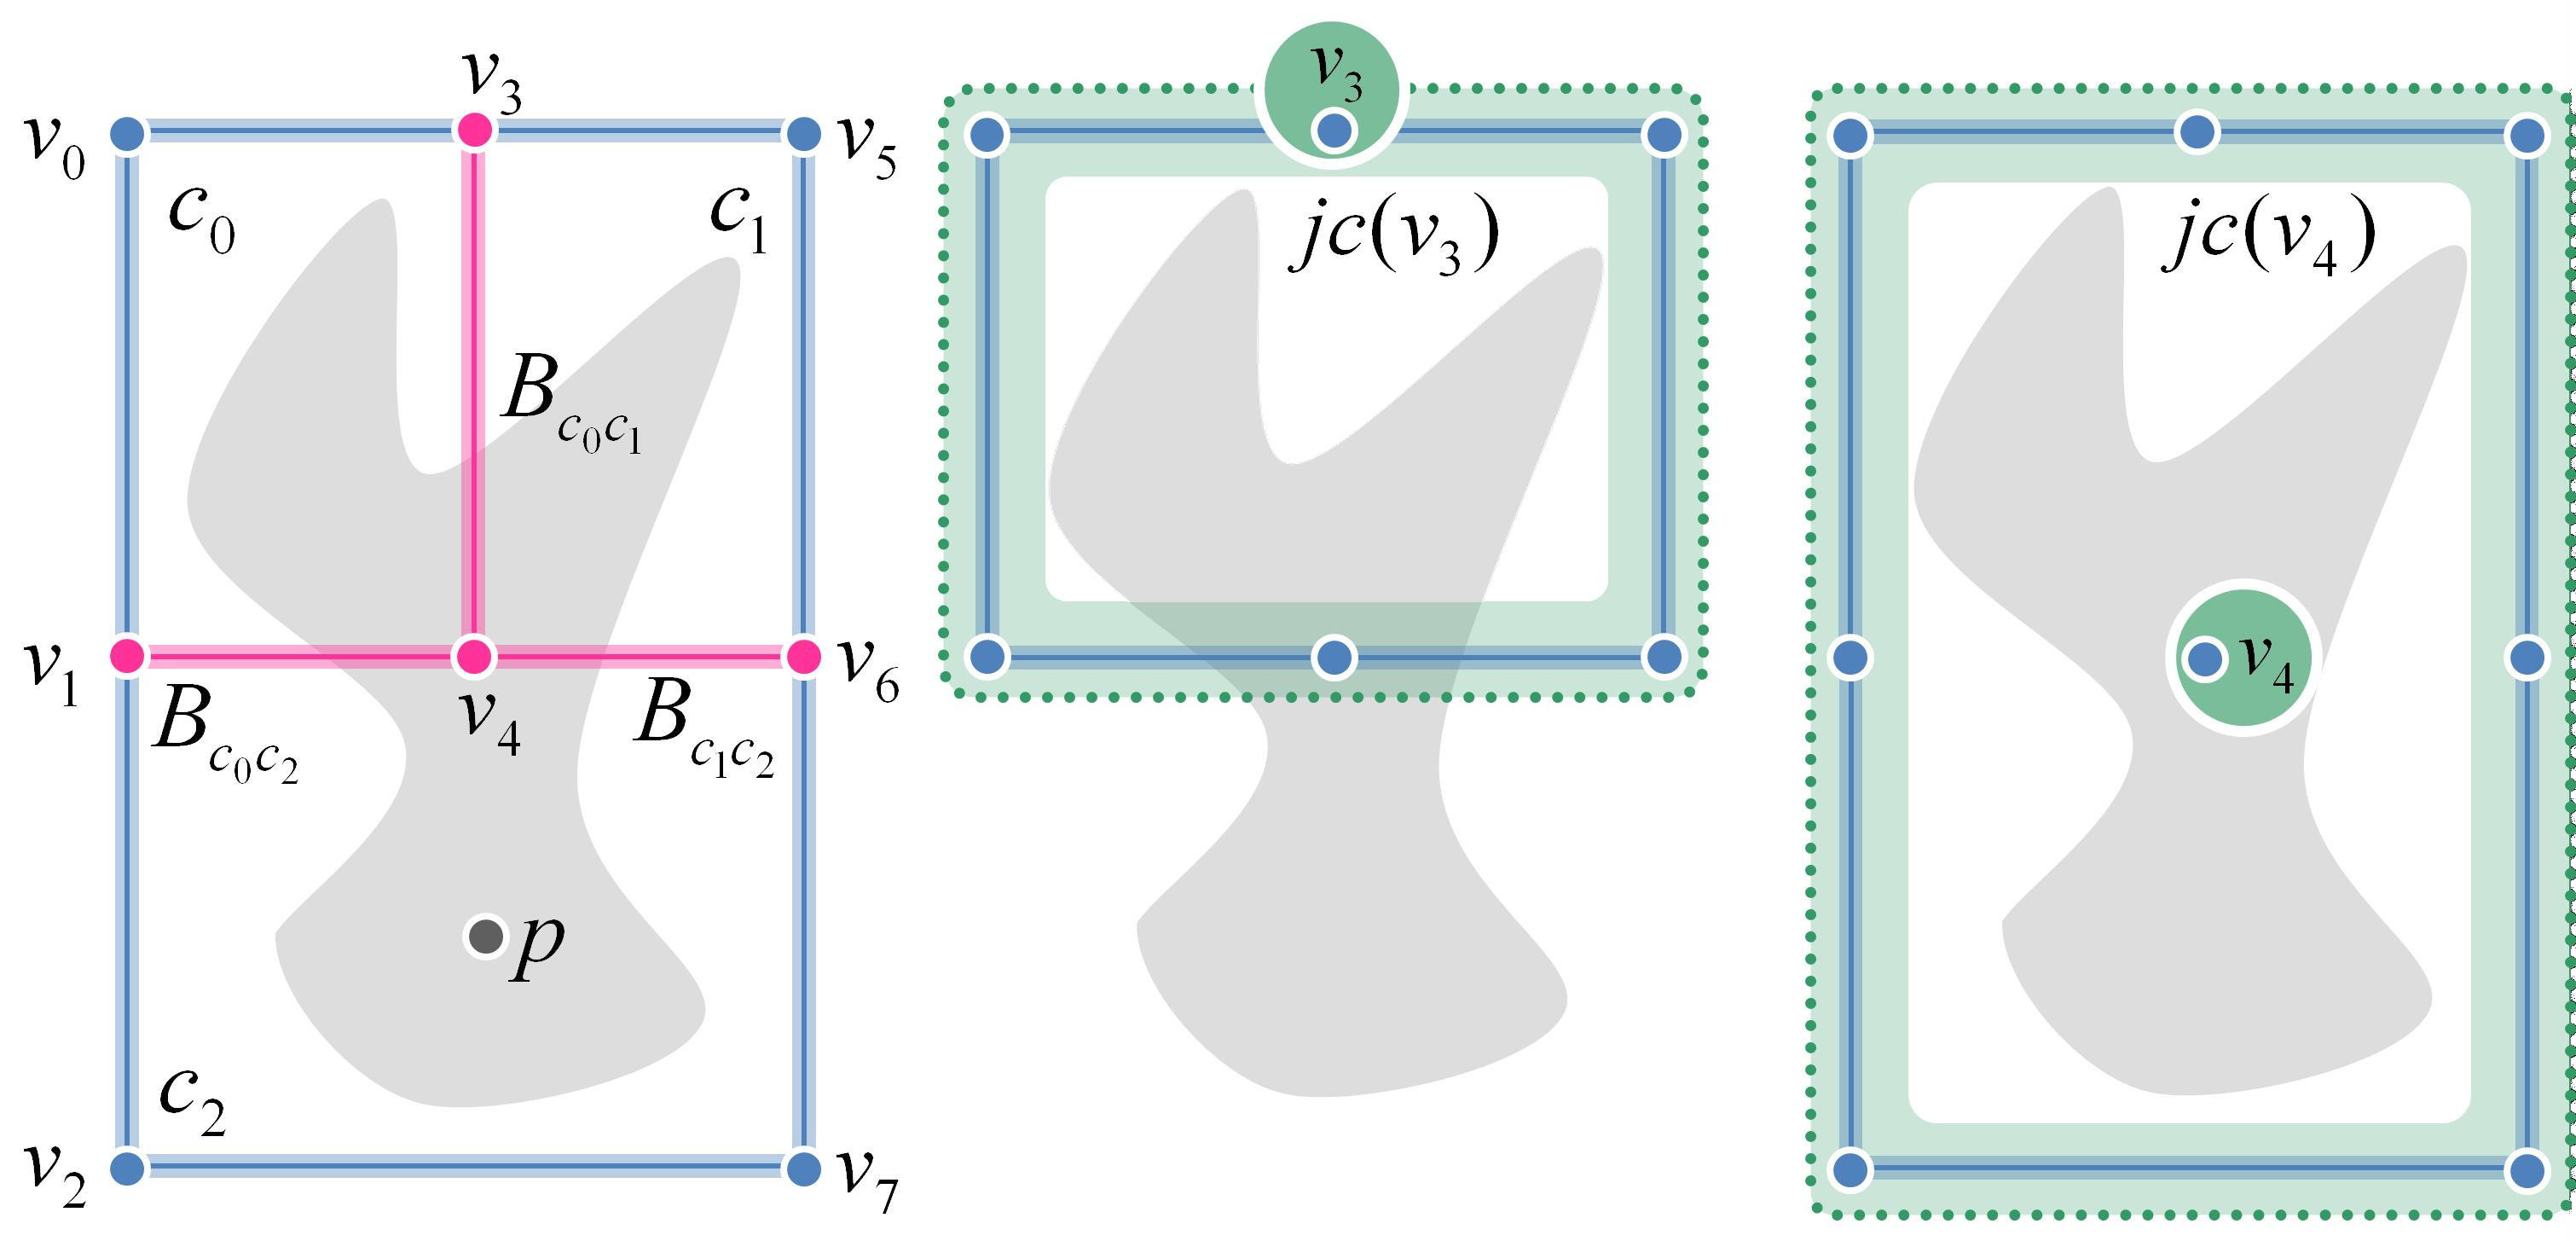
\includegraphics[scale=0.07]{joinCages}
    \end{center}
    \caption{\citep{GPCP13}}
  \end{figure}
\end{frame}

\begin{frame}{*Cages $_{\text{\citep{GPCP13}}}$}
  \begin{alertblock}{Points négatifs :}
    \setbeamercolor{itemize item}{fg=MRed}
    \begin{itemize}
    \item Nombreuses fonctions imbriquées
    \item Utilisation de coordonnées harmoniques
    \end{itemize}
  \end{alertblock}
  \begin{exampleblock}{A retenir :}
    \setbeamercolor{itemize item}{fg=MGreen}
    \begin{itemize}
    \item Déformations localisées et lisses
    \item Différentes méthodes de calcul des coordonnées
    \end{itemize}
  \end{exampleblock}
\end{frame}

\section{\scshape Méthode proposée}

\begin{frame}{Méthode proposée}
  \begin{block}{Idée}
    \begin{itemize}
    \item Coordonnées barycentriques sont définies dans $\mathbb{R}^2$
    \item Zone d'influence autour d'une cage
    \item Estompement progressif des coordonnées au bord
    \item Mélanger les coordoonnées aux zones de rencontre
    \end{itemize}
  \end{block}
  \begin{figure}[h]
    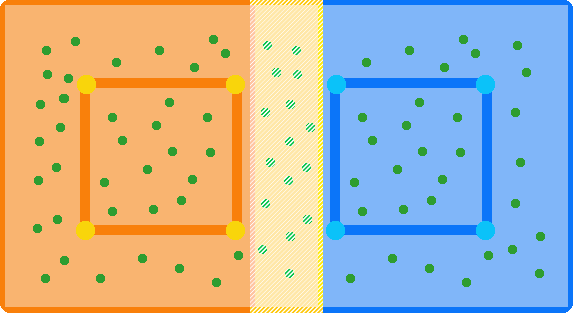
\includegraphics[scale=0.2]{bordure-cage}
  \end{figure}
\end{frame}

\begin{frame}{Méthode proposée}
  \begin{alertblock}{Points clés}
    \setbeamercolor{itemize item}{fg=MRed}
    \begin{itemize}
    \item Coordonnées MVC seulement $C^0$ autour des sommets
    \item Mélanger les différentes positions calculées de façon lisse
    \end{itemize}
  \end{alertblock}
\end{frame}

%%%%%%%%%%%%%%%%%%%%%%%%%%%%%%%%%%%%%%%%%%%%%%%%%%%%%%
%%%%%%%%%%%%%%%%%%%%%%%%%%%%%%%%%%%%%%%%%%%%%%%%%%%%%%
\section{\scshape Suite du stage}
\begin{frame}{Suite du stage}
  A court terme
  \begin{itemize}
  \item Corriger les problèmes de continuité des MVC
    $_{\text{\citep{LS08}}}$
  \item Etude des outils à base de courbes
  \end{itemize}
  A "long" terme
  \begin{itemize}
  \item Gestion des différents niveaux de résolution $_{\text{\citep{Hur12}}}$
  \item Généralisation de la technique de mélange aux outils de
    différentes dimensions
  \end{itemize}
\end{frame}

\begin{frame}{}
\begin{center}
\huge Merci de votre attention.
\end{center}
\end{frame}

\appendix

\end{document}

%%% Local Variables: 
%%% mode: latex
%%% LaTeX-command: "latex -shell-escape"
%%% End: 